\chapter{Projekt systemu}\label{chap:projekt}

W tym rozdziale został przedstawiony zamysł członków zespołu na opracowywaną grę. Stanowi on opis pożądanych rezultatów,
do których zespół będzie dążyć w trakcie implementacji. Kolejno zostały opisane oczekiwane działanie poszczególnych
mechanik, z których będzie się składał ostateczny produkt. 

\section{Organizacja (Bartosz Strzelecki)}\label{s:org}
W tym podrozdziale przedstawiono harmonogram prac, wraz z ich przewidywanym terminem realizacji.
Ponadto zaprezentowano skład zespołu projektowego, kompetencje ich członków oraz podział zadań.
\subsection{Główne etapy projektu}
\begin{center}
  \begin{tabular}{| m{30em} | m{12em}|} 
  \hline
  Etap & Termin realizacji \\
  \hline\hline
  Wybór i analiza konkretnego kontekstu historycznego. & Kwiecień 2023 \\
  \hline
  Syntetyczny opis modelu postrzegania przestrzeni na podstawie dzieł pisanych, architektury i sztuki. & Kwiecień — Maj 2023 \\
  \hline
  Przegląd rozwiązań stosowanych w grach strategicznych z wybranego okresu oraz dodatkowo mechanizmów z innych gier, które mogłyby być zaadoptowane na potrzeby projektu. & 2, 3 kwartał 2023 \\
  \hline
  Opracowanie fabuły, selekcja postaci i wydarzeń, a także określenie zakresu autonomii świata gry oraz możliwości modyfikowania go przez gracza. & Czerwiec 2023 \\
  \hline
  Opracowanie szczegółowej koncepcji i projektu gry, w tym projekt mechanizmów zawartych w prototypie. & Lipiec 2023 \\
  \hline
  Implementacja poszczególnych funkcjonalności gry. & 4 kwartał 2023 \\ 
  \hline
  Testowanie, weryfikacja założeń i walidacja. & Listopad — Grudzień 2023 \\
  \hline
  Stworzenie dokumentacji przeprowadzonych prac. & 3, 4 kwartał 2023 \\
  \hline
\end{tabular}
\end{center}
Przewidywany termin zakończenia prac nad projektem to grudzień 2023 roku.
\begin{figure}[htbp]
    \centering
    \includegraphics[width=1\textwidth]{uml/Harmonogram}
    \caption{Harmonogram przedstawiony w postaci diagramu gantt.}
\end{figure}
\break
\section{Skład zespołu projektowego}
\begin{center}
  \begin{tabular}{ | m{10em} || m{10em} | m{10em} | m{10em} | }
    Imię i nazwisko & Bogna Lew & Zofia Sosińska & Bartosz Strzelecki \\
  \hline\hline
    Numer indeksu & 184757 & 184896 & 184529 \\
  \hline
    %%Kompentencje & Posiada & Posiada & Posiada \\
    Zadania & System budowania, sterowanie postacią & Interfejs użytkownika & Sztuczna inteligencja postaci\\
  \hline
  \end{tabular}
\end{center}

\section{Analiza i specyfikacja wymagań (Bogna Lew)}\label{s:wymagania}
W niniejszej sekcji przedstawiono specyfikę wymagań funkcjonalnych, pozafunkcjonalnych oraz tych, wynikających z
głównych założeń projektu. Dodatkowo zawiera ona diagramy przypadków użycia, maszyny stanów oraz klas prototypowej gry.

\subsection{Specyfika wymagań wynikających z założeń projektu}
“Starożytni świat widzieli inaczej, mniej płasko”\cite{gbobrektvgry}. Dobrze obrazującym ówczesne postrzeganie
przestrzeni przykładem jest mapa Imperium Rzymskiego, pokazana na \ref{fig:mapaIR}. Czytanie jej dosłownie mija się z
celem. Nie są na niej zachowane ani proporcje, ani strony świata. Mimo tego, że basen Morza Śródziemnego został
ówcześnie dosyć dokładnie oddany, “nie wydaje się, aby Rzymianom współczesna kartograficzna wierność była potrzebna”\cite{gbobrektvgry}.
“Dowódcy opierali się na swojej wiedzy, wiedzy wynajętych przewodników oraz informacjach zwiadowców i tubylców”\cite{gbobrektvgry}.

\begin{figure}[htbp]
    \centering
    
\includegraphics[width=0.5\textwidth]{images/mapaIR.png}
    \caption{Mapa basenu Morza Śródziemnego z czasów Imperium Rzymskiego}\label{fig:mapaIR}
\end{figure}

Z punktu widzenia projektu kluczowe jest jak najdokładniejsze oddanie realiów historycznych przy jednoczesnym
uwzględnieniu jakości rozgrywki gracza oraz cech charakterystycznych dla gier typu RTS. Z założeń wynika, że fabuła
gry powinna zostać osadzona w czasach sprzed wielkich odkryć geograficznych. Na tej podstawie zostały zdefniowane
dodatkowe wymagania, które powinien spełniać prototyp:
\begin{itemize}
  \item Sposób nawigacji powinien jak najdokładniej odpowiadać temu stosowanemu w wybranej epoce;
  \item Postacie w grze powinny stylistycznie pasować do realiów historycznych;
  \item Postacie powinny posługiwać się słownictwem adekwatnym do czasów, w których osadzona jest gra;
  \item Postacie powinny jak najlepiej oddawać światopogląd w danych czasach;
  \item Oręż stosowany w grze powinien odpowiadać realiom historycznym;
  \item Budowle w grze powinny stylistycznie odpowiadać wybranej epoce;
  \item Sposób komunikacji z postaciami powinien imitować ten stosowany w danych czasach;
\end{itemize}

\subsection{Wymagania funkcjonalne}\label{ss:fun}
W przedstawionej liście zostały wymienione wymagania funkcjonalne, które powinien spełniać prototyp gry.

\begin{itemize}\label{list:fun}
  \item Zapis oraz odczyt wybranego stanu gry lokalnie na komputerze użytkownika;
  \item Uruchomienie nowej gry;
  \item Możliwość sterowania postacią gracza;
  \item Możliwość nawigacji w świecie gry;
  \item Możliwość wchodzenia w interakcję z postaciami niezależnymi;
  \item Możliwość przyjmowania zleceń od postaci niezależnych;
  \item Możliwość najmowania postaci wojowników;
  \item Możliwość wydawania komend wynajętym postaciom;
  \item Możliwość zlecania budowy;
  \item Możliwość zdobywania zasobów;
\end{itemize}

\subsection{Wymagania pozafunkcjonalne}\label{ss:nonfun}
Poniższa lista przedstawia wymagania niefunkcjonalne projektu.

\begin{itemize}\label{list:nonfun}
  \item Rozgrywka w trybie offline;
  \item Działanie na urządzeniach z systemem Windows lub Linux;
  \item Dostosowywanie rozmiaru do wielkości ekranu komputera użytkownika;
  \item Obsługa klawiatury oraz myszy;
  \item Działanie w czasie rzeczywistym;
\end{itemize}

\subsection{Diagram przypadków użycia}\label{ss:usecase}
Niniejsza sekcja przedstawia diagram przypadków użycia dla głównych funkcjonalności, które będzie zawierać prototypowa gra.
Opisuje on przewidywane usługi oferowane przez poszczególne mechaniki programu.

Jedną z głównych akcji, które gra udostępnu jest wydanie rozkazów przyjaznym jednostkom. Polega ona na poinformowaniu
wojowników przez gracza jaką czynność powinni w danym momencie wykonać. Kolejną możliwością jest zlecenie budowy, czyli
poelceniu postaci budowniczego wybudowania wybranego obiektu w określonym przez gracza miejscu. Ponadto użytkownik
będzie mógł przeprowadzać rozmowy z postaciami niezależnymi. Oznacza to, że będzie mógł zainicjować z nimi dialog i
następnie kształtować jego przebeig poprzez wybieranie swoje odpowiedzi z opcji proponowanych przez grę.

\begin{figure}[!htbp]
    \centering
    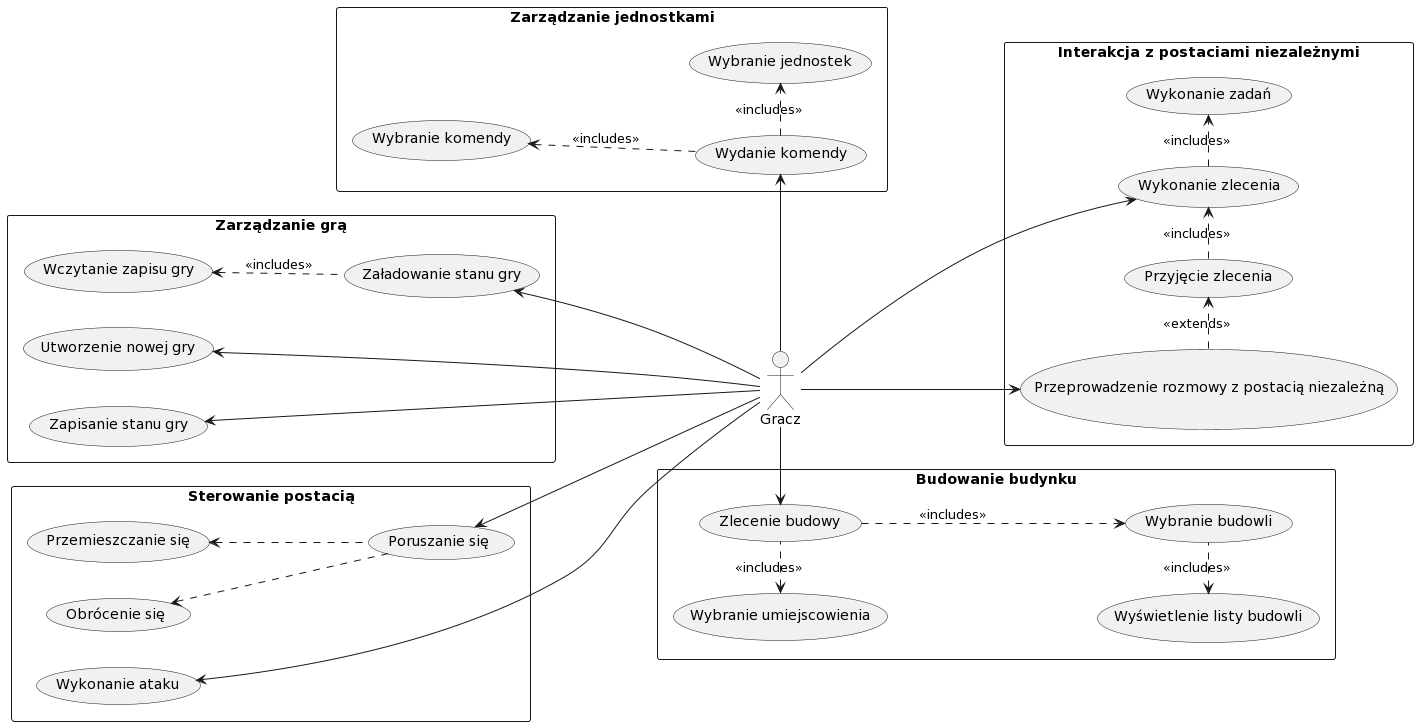
\includegraphics[width=1.0\textwidth]{images/diagrams/usecase.jpg}
    \caption{Diagram przypadków głównych mechanik gry.}\label{fig:usecases}
\end{figure}
\FloatBarrier

\subsection{Diagram stanów}\label{ss:state}
W tym podpunkcie został przedstawiony diagram stanów prototypowej gry, który ukazuje jej przewidywany sposób działania.
Prezentuje on podstawowe stany, w których może się znaleźć system gry.

Do podstawowych stanów należą "Menu główne" oraz "Rozgrywka". Pierwszy z nich oznacza, że program został uruchomiony, a
gracz wyświetla panel główny. Z tego stanu możliwe jest przejście do stanów "Odczytanie stanu gry" bądź "Utworzenie
nowej gry", które to powodują rozpoczęcie gry z zapisu lub od początku.

Stan "Rozgrywka" jest stanem złożonym i określa, że gra została rozpoczęta. W jego skład wchodzą przede wszytskim takie
stany jak "Interakcja z postacią niezależną", w którym program się znajdzie gdy gracz rozpocznie dialog z postacią w grze,
czy "Zarządzanie jednostkami", który to oznacza, że użytkownik wydaje rozkazy swoim wojownikom.

Diagram stanów został przedstawiony na rysunku \ref{fig:states}.

\begin{figure}[!htbp]
    \centering
    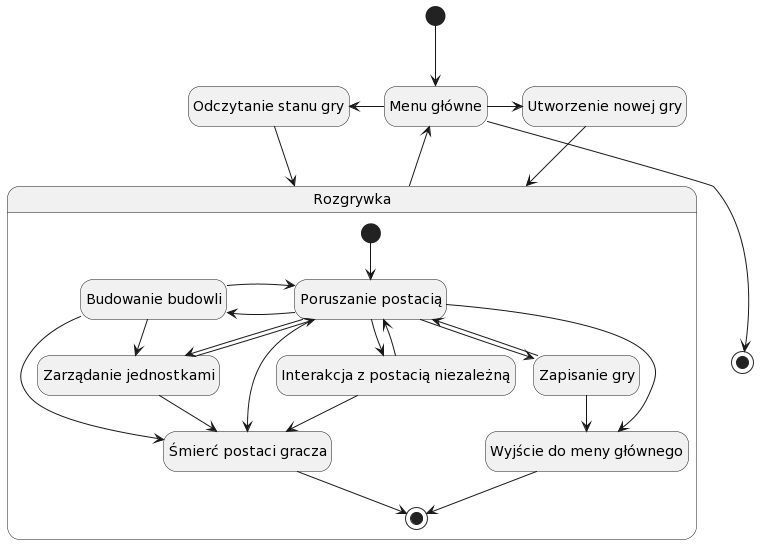
\includegraphics[width=1.0\textwidth]{images/diagrams/state.jpg}
    \caption{Diagram stanów gry.}\label{fig:states}
\end{figure}
\FloatBarrier

\subsection{Diagram klas}\label{ss:class}
W tej sekcji został pokazany uproszczony diagram klas (rys. \ref{fig:classes}), przedstawiający główne elementy gry.
Obrazuje podstawową strukturę tworzonego systemu oraz zależności pomiędzy poszczególnymi komponentami.

Do najważniejszych klas należą "Interfejs użytkownika", "Mechanizm interakcji z postaciami", "Mechanizm zarządzania
jednostkami" oraz "Mechanizm budowania". Obrazują one podstawowe komponenty gry, których głównym zadaniem jest zarządzanie
poszczególnymi mechanikami. "Interfejs użytkownika" jest odpowiedzialny za interakcję z graczem oraz pomaganie mu w
trakcie rozgrywki. Pozostałe trzy odpowiadają kolejno za umożliwienie graczowi na prowadzenie dialogów z postaciami
niezależnymi, wydawanie komend jego zaprzyjaźnionym jednostkom oraz budowanie obiektów.
\begin{figure}[!htbp]
    \centering
    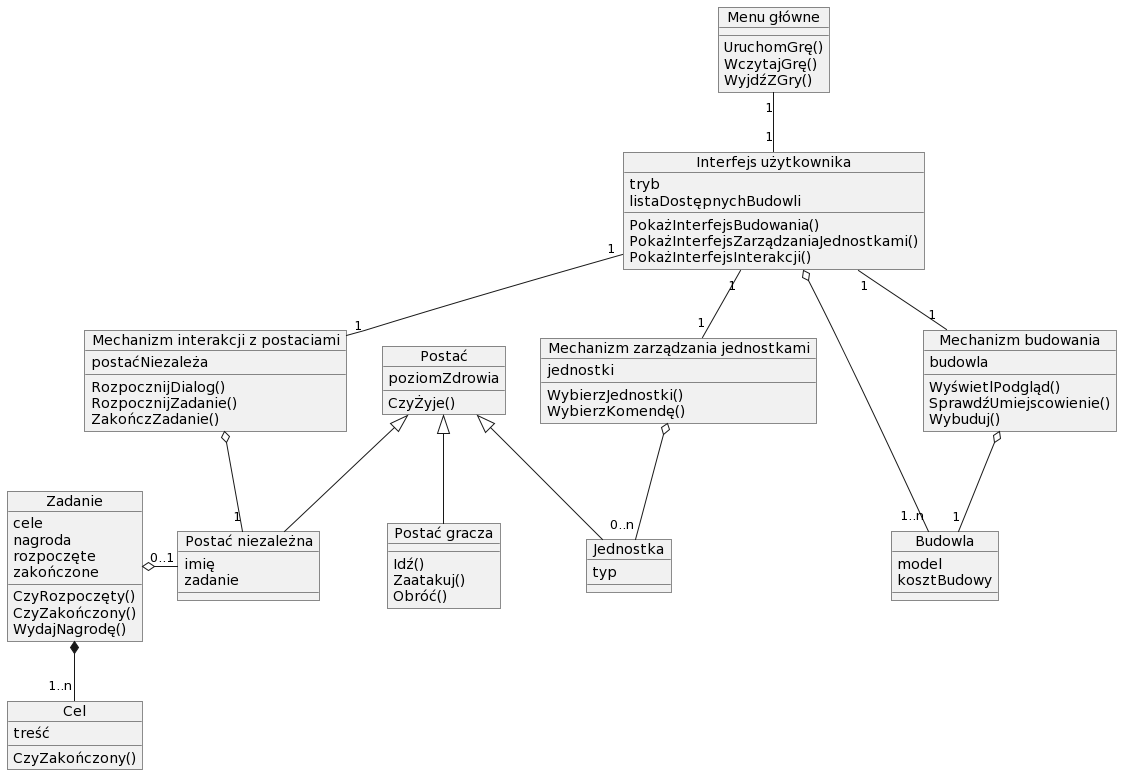
\includegraphics[width=1.0\textwidth]{images/diagrams/class.jpg}
    \caption{Diagram klas gry.}\label{fig:classes}
\end{figure}
\section{Opis świata gry (Bogna Lew)}
Fabuła wytwarzanej gry ma zostać osadzona w realiach wczesnośredniowiecznych. Została ona zainspirowana Celtami, których
w tym okresie można było spotkać głównie w Irlandii. Z tego powodu mapa świata gry będzie prezentować górzystą wyspę, na
której gracz będzie mógł znaleźć niewielką wioskę oraz obozowiska.

Graczowi udostępniona zostanie jego własna postać do bezpośredniego sterowania. Takie rozwiązanie "czyni gracza
kreatywnym elementem działajacym wewnątrz dyskursu, który posiada przestrzenny charakter"\cite{olbrzymwcieniu}. Typowym
elementem gry są zadania poboczne, czasem pośrednio związane z głównym celem gry. Stanowi to urozmaicenie rozgryki i
dodatkowo zachęca gracza do zagłębiania się w nią. "W odniesieniu do gier komputerowych można więc mówić o podwójnym
motywowaiu ich użytkowników, które dokonuje sie na dwóch narracyjnych poziomach: jedna z motywacji wyznacza cel całej
rozgrywce, druga natomiast jest ulokowana w przestrzeni pojedynczej misji i kończy wraz z jej zakończeniem"\cite{olbrzymwcieniu}.
Z tego powodu trakcie gry użytkownik będzie mógł spotkać postaci niezależne, z którymi możliwe będzie wejście w interakcje, kończące
się np. zleceniem wykonania zadania. W ich realizacji będą mu pomagać jednostki, z którymi się zaprzyjaźni w trakcie
rozgrywki i którym będzie mógł wydawać komendy zgodnie z ich typem. Dodatkowo w trakcie eksploracji świata natrafi na
nieprzyjazne postacie, z którymi będzie toczyć walki. Grę urozmaicą postaci zwierząt, które mogą być neutralne, bądź
agresywne wobec gracza.

Gra będzie udostępniać trzy podstawowe surowce, za które gracz będzie mógł budować budynki. Przewidywane są dwa sposoby
ich pozyskiwania. Pierwszym z nich jest wykonywanie zadań, za które może uzyskać nagrody w postaci pewnej ilości
surowców. Kolejnym sposobem jest zbieranie kłód drewna oraz kamieni leżących na ziemi. Podnoszenie ich dostarczy
jednorazowy przypływ odpowiadającego im zasobu.

\section{Kontroler postaci. Bogna Lew}

W trakcie rozgrywki istotnym aspektem wpływającym na jakość jest mechanizm sterowania postacią. Z tą mechaniką gracz ma
bezpośredni kontakt, ponieważ to właśnie za jej pomocą może eksplorować świat.

Do implementacji tego mechanizmu zainspirowaliśmy się grą Skyrim. Postać jest sterowana za pomocą klawiszy “w”, “a”, “s”
oraz “d”, natomiast jej rotacja oraz obrót kamery jest kontrolowany przez mysz. Całość została podzielona na cztery
części.

Pierwsza z nich odpowiada za przemieszczanie się postaci. Do tego wykorzystuje Input Manager, w którym zostały
zmapowane odpowiednie klawisze dla każdej z osi, wzdłuż której gracz może się przemieszczać. W rezultacie powstały dwa
kierunki - przód/tył oraz prawo/lewo. Naciśnięcie odpowiedniego przycisku skutkuje zwróceniem wartości 1 bądź -1, które
symbolizują zwrot wektora przemieszczenia wzdłuż osi. Na tej podstawie wyznaczane jest faktyczne przesunięcie postaci
względem kierunku, w którym jest zwrócona oraz modyfikowane jest jej położenie. Dodatkowo ten komponent odpowiada za
wyznaczenie prędkości, z jaką gracz się porusza. Domyślnie postać przemieszcza się tempem chodu, jednakże jeśli gracz
przytrzyma lewy klawisz Shift, to zacznie się poruszać biegiem.

Druga część kontrolera odpowiada za ustawienie odpowiedniej animacji. Do tego wykorzystuje ona wartości zwrotu wzdłuż
obu osi oraz prędkość, które są wyznaczane w poprzednim komponencie. Na ich podstawie wyznacza kolejne części nazwy
animacji, po czym, jeśli jest inna niż aktualnie wyświetlana, uruchamia ją.

Kolejny komponent nadzoruje rotację postaci oraz co za tym idzie - kamery. Analogicznie wykorzystywany jest Input
Manager, jednak w tym przypadku przechwytywane jest przesunięcie myszy. Komponent udostępnia graczowi możliwość
sterowania kierunkiem, w którym postać patrzy, a co za tym idzie - względem którego się przemieszcza. Jednocześnie
następuje dostosowanie położenia kamery tak, aby zawsze patrzyła w tym samym kierunku co postać gracza. Ponadto
komponent umożliwia przesunięcie kamery po łuku do góry bądź do dołu. Dzięki temu gracz może dokładniej zobaczyć
co znajduje się nad oraz tuż przed nim.

Ostatni komponent odpowiada za kontrolowanie przybliżania kamery. W tym celu w Input Managerze zostało zamapowane kółko
myszy. Zwrócona przez system wartość jest wykorzystywana do obliczenia odległości kamery od postaci przy zachowaniu
ustalonych przez grę ograniczeń. Dodatkowo, komponent dokonuje również automatycznego przybliżania, jeśli wskutek
przemieszczania się postaci, pomiędzy nią, a kamerą miałaby się znaleźć przeszkoda. Dzięki temu nie zostanie zasłonięty
widok tego co się dzieje wokół postaci. Odsunięcie się od przeszkody zaskutkuje oddaleniem kamery do poprzedniej
odległości.

\section{Interfejs użytkownika (Zofia Sosińska)}\label{chap:ui}
Interfejs użytkownika (ang. user interface, UI) jest to zbiór najważniejszych informacji przedstawiony graczowi w sposób czytelny. Może się to odbywać za pomocą na przykład obrazków, tekstów, czy wskaźników. Dzięki UI możliwy jest wgląd w aktualny stan wiedzy grywalnej postaci. 

Projekt interfejsu użytkownika przewiduje trzy tryby: zwykły, budowania oraz walki. Zadaniem każdego z nich będzie odzwierciedlenie aktualnej wiedzy granej postaci z naciskiem na najpotrzebniejsze w danej chwili informacje.
	
\subsection{Interfejs podstawowy}
Interfejs podstawowy przewiduje funkcje, takie jak pokazanie:
\begin{itemize}
    \item surowców i funduszy,
    \item aktualnego czasu w grze, 
    \item kompasu,
    \item informacji o możliwym  rozpoczęciu konwersacji z inną postacią;
\end{itemize}
Inspiracją dla górnego paska z informacjami jest ten użyty w grze Warcraft 3. Prostota i surowość stylu będą współgrać z klimatem gry.

W naszej grze skupimy się jednak na tym, aby interfejs użytkownika zabierał jak najmniej miejsca. Dlatego też projekt zakłada, że poszczególne obiekty nie będą ze sobą połączone, a jedynie “dryfować” w przestrzeni.
Jako ważny element tej części UI zawarty zostanie kompas, wzorowany na tym z gry The Elder Scrolls V: Skyrim.


Szacowany projekt interfejsu podstawowego UI wyświetlono na rysunku \ref{fig:ui_main} .
\begin{figure}[htbp]
    \centering
    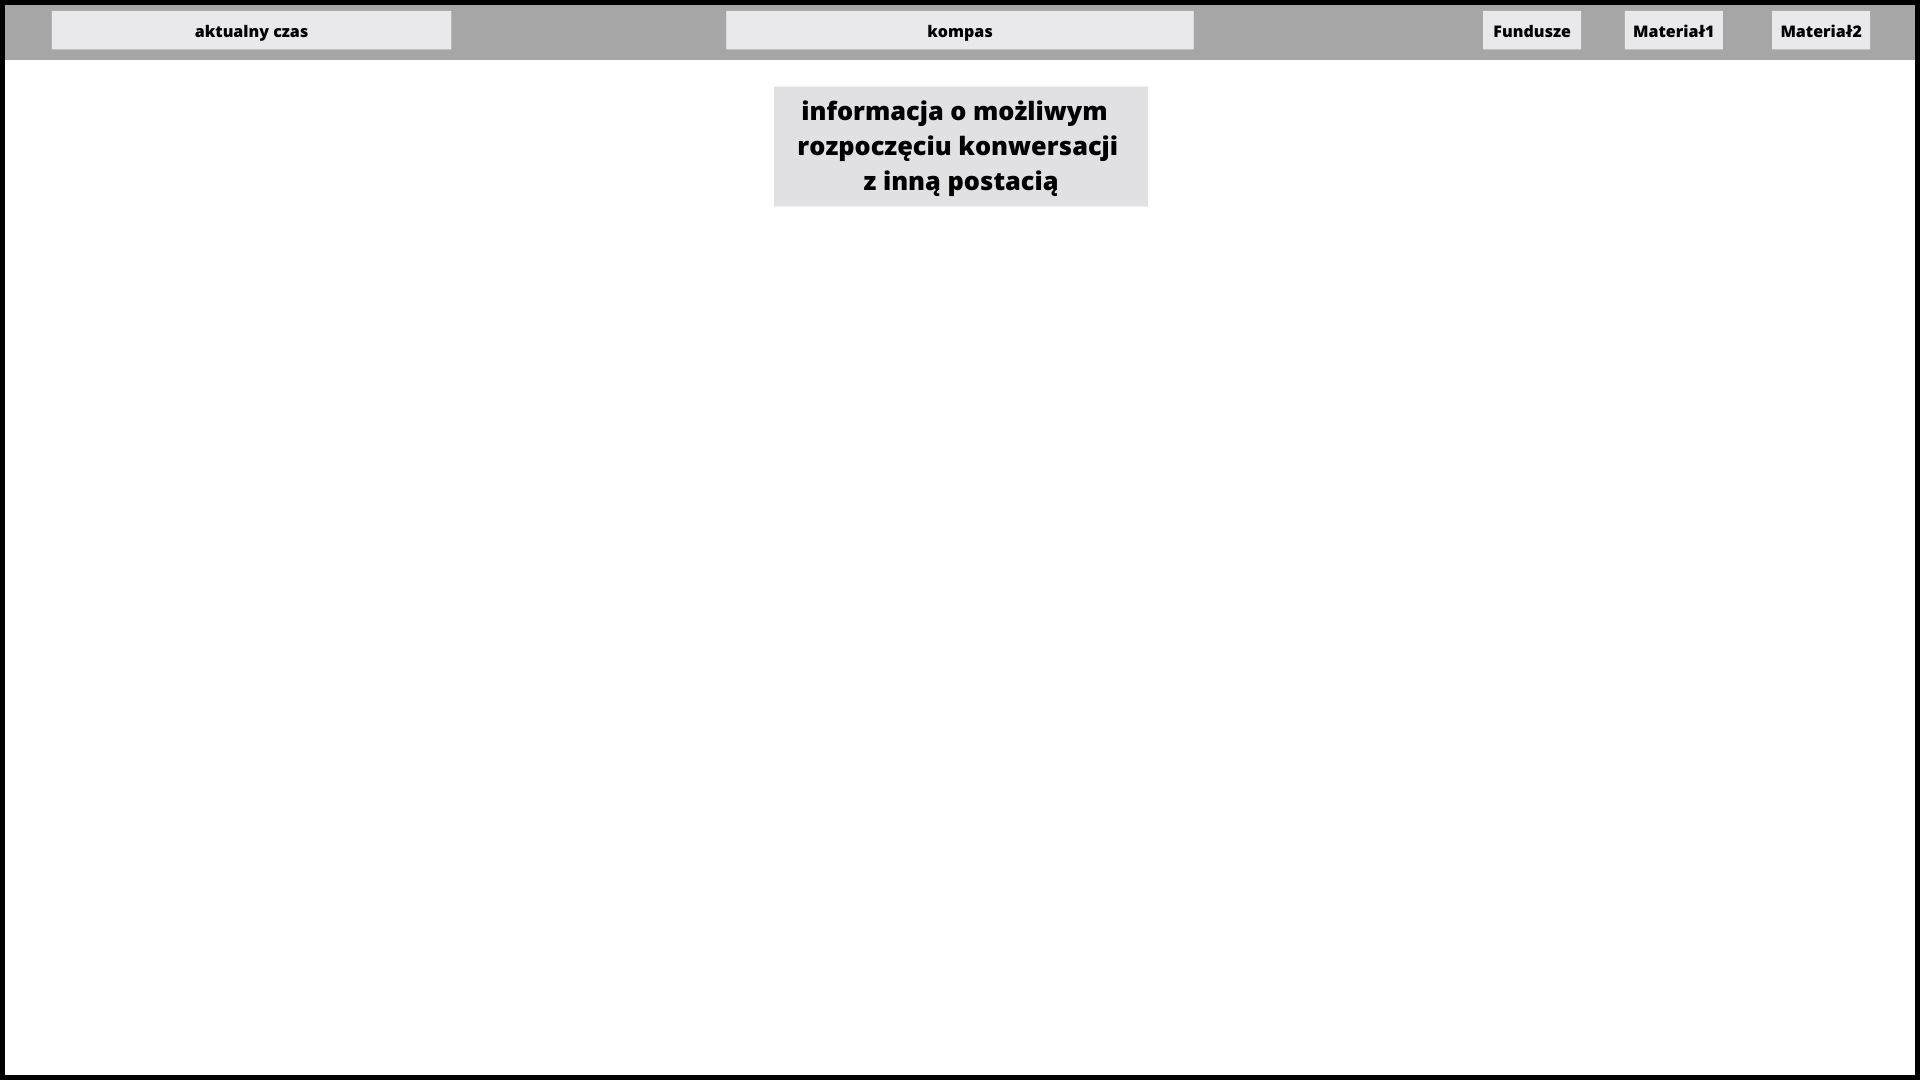
\includegraphics[width=0.9\textwidth]{images/ui/ui_proj_ogolne.jpg}
    \caption{Projekt interfejsu podstawowego UI.
    }\label{fig:ui_main}
\end{figure}
 
\subsection{Menu stawiania budynków}
 W menu stawiania budynków informacje wcześniej przedstawione zostaną na ekranie. Dodatkowo pokażą nam się dostępne do zbudowania budynki, a po wybraniu pojawią się przed nami. Po zatwierdzeniu budynek zostanie wybudowany.
	Inspiracją do przedstawienia dostępnych budowli jest rozwiązanie gry Orcs must die!


    Szacowany projekt trybu budowania UI wyświetlono na rysunku \ref{fig:ui_bud} .
    \begin{figure}[htbp]
        \centering
        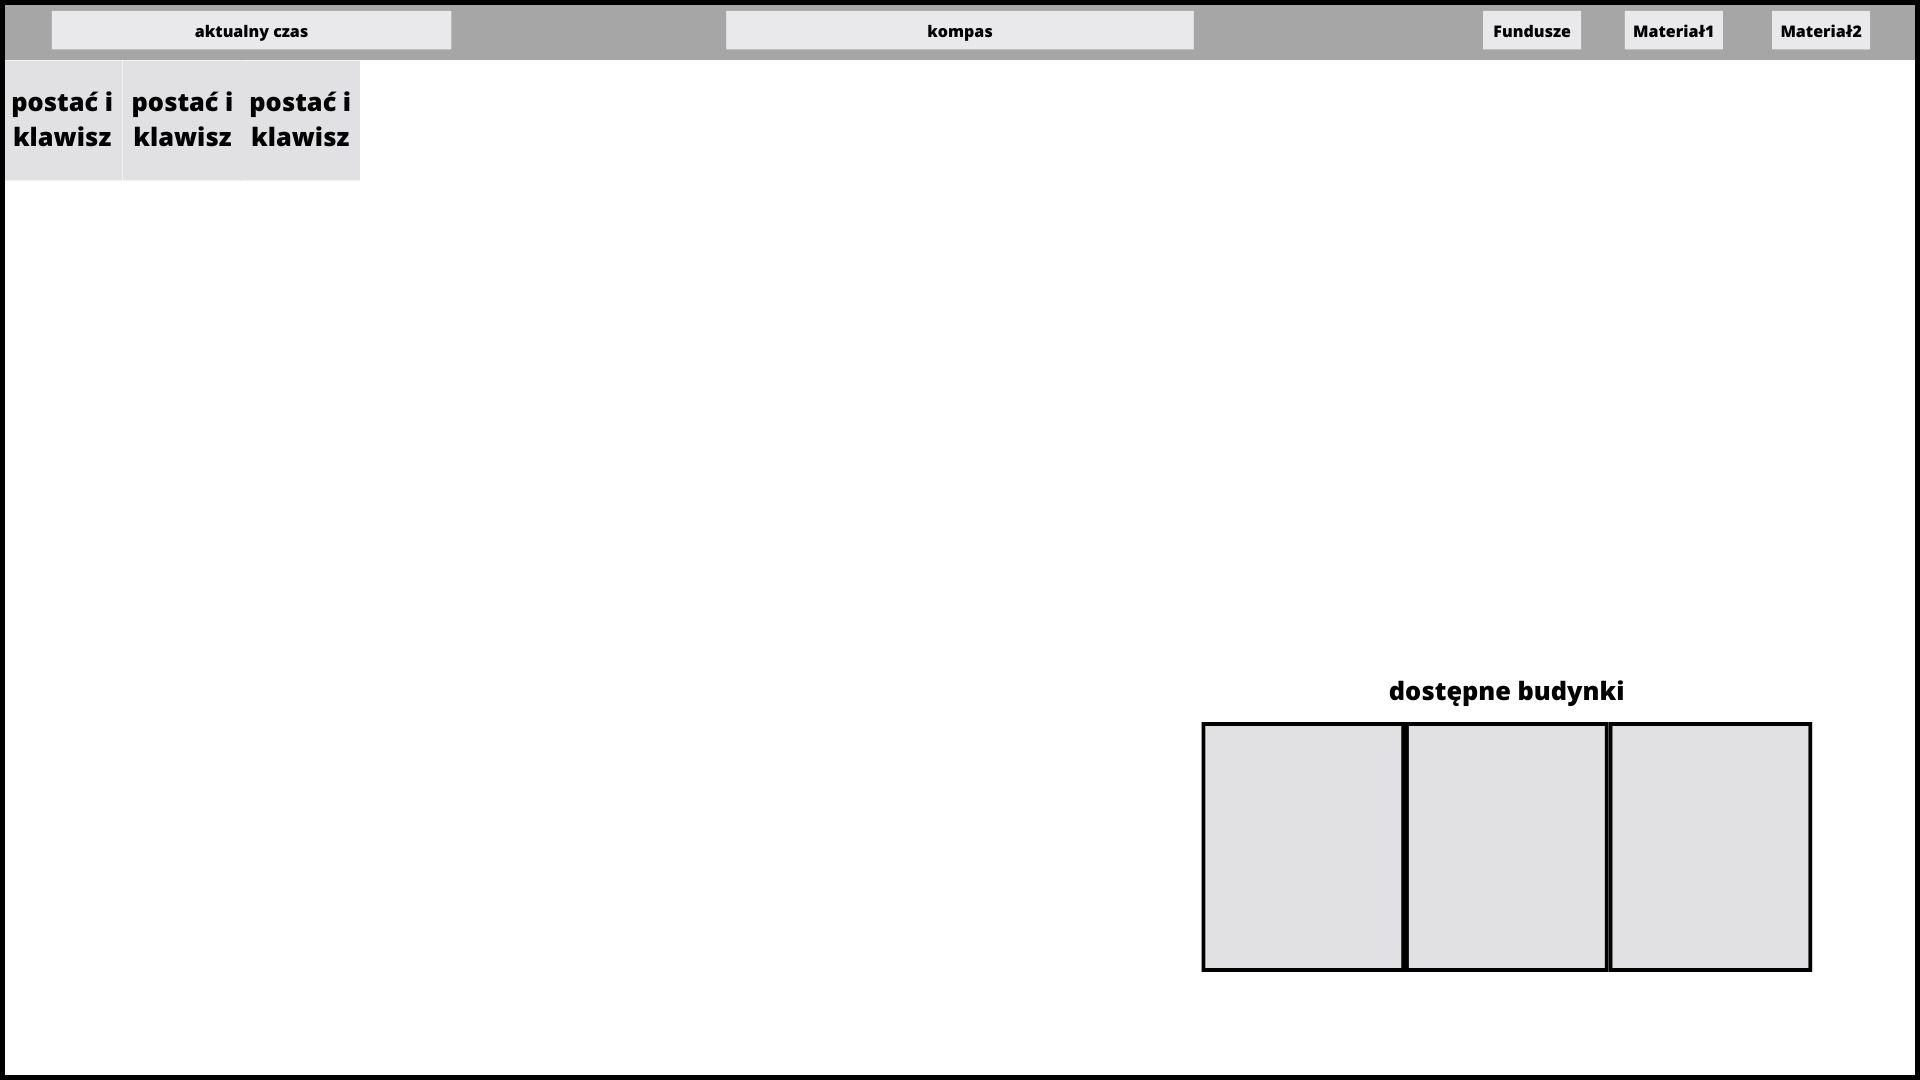
\includegraphics[width=0.9\textwidth]{images/ui/ui_proj_budowanie.jpg}
        \caption{Projekt menu stawiania budynków UI.
        }\label{fig:ui_bud}
    \end{figure}


\subsection{Tryb walki}
Bliźniaczo do trybu budowania, gdy rozpocznie się walka, podstawowe informacje zostają na ekranie, a dodatkowo gracz dostaje informacje o dostępnych rozkazach do wydania. Nasze rozwiązanie będzie podobne do pomysłu z gry Mount\&Blade.

Szacowany projekt trybu budowania UI wyświetlono na rysunku \ref{fig:ui_wal} .
    \begin{figure}[htbp]
        \centering
        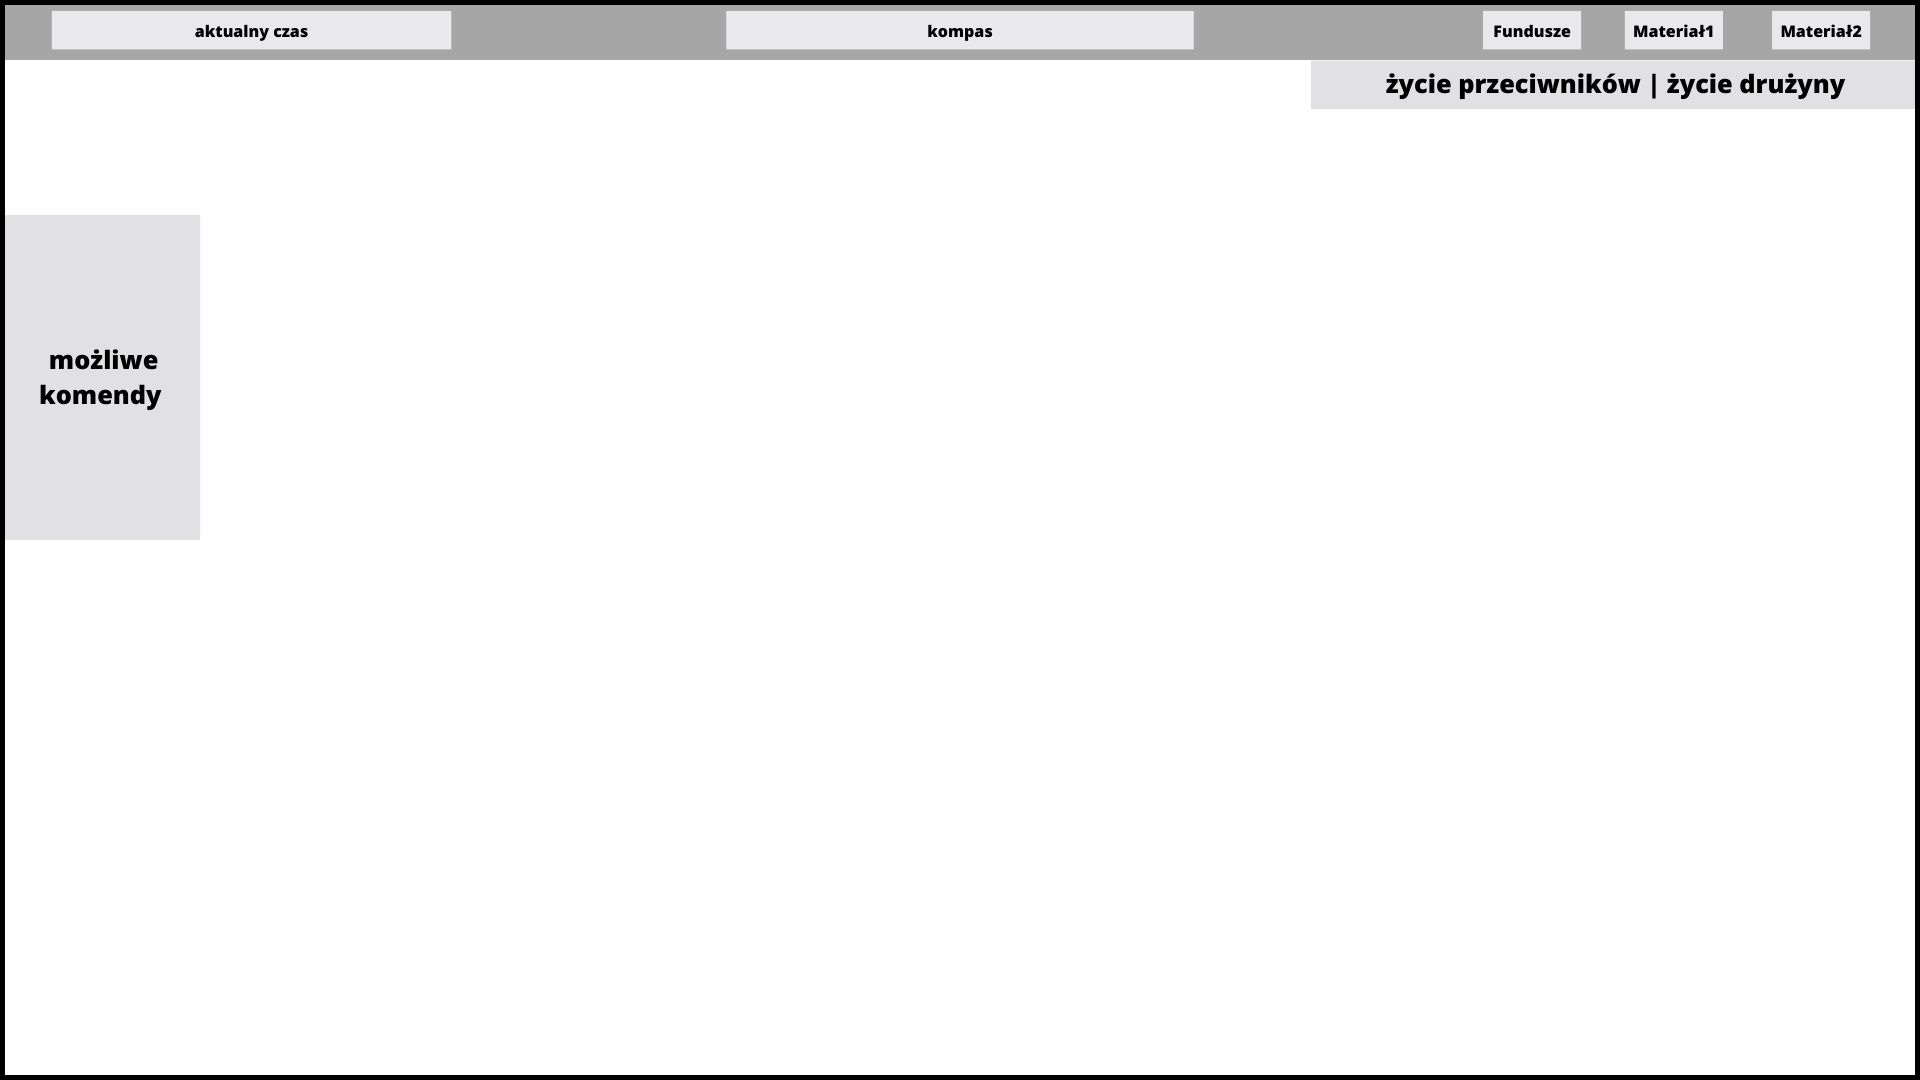
\includegraphics[width=0.9\textwidth]{images/ui/ui_proj_walka.jpg}
        \caption{Projekt trybu walki UI.
        }\label{fig:ui_wal}
    \end{figure}

\section{Menu główne (Zofia Sosińska)}\label{chap:menu_main}
Pierwsze co zobaczy użytkownik po włączeniu programu to menu główne, więc jego zadaniem będzie oddanie klimatu programu,
umożliwienie rozpoczęcia rozgrywki oraz zamknięcie aplikacji.
Projekt zakłada, że menu główne udostępni kluczowe funkcjonalności za pomocą przycisków:
\begin{itemize}
    \item rozpoczęcia nowej gry,
    \item wczytania zapisanej gry,
    \item wyjścia z programu.
\end{itemize}

Przycisk wczytania gry będzie musiał pozwolić na wybranie pliku zapisu. W tym celu przewiduje się wyświetlenie listy
z możliwością przewijania treści za pomocą suwaka. Jej elementami będą przyciski z nazwą zapisu, których naciśnięcie przeniesie 
użytkownika do konkretnego stanu gry.

\begin{figure}[htbp]
    \centering
    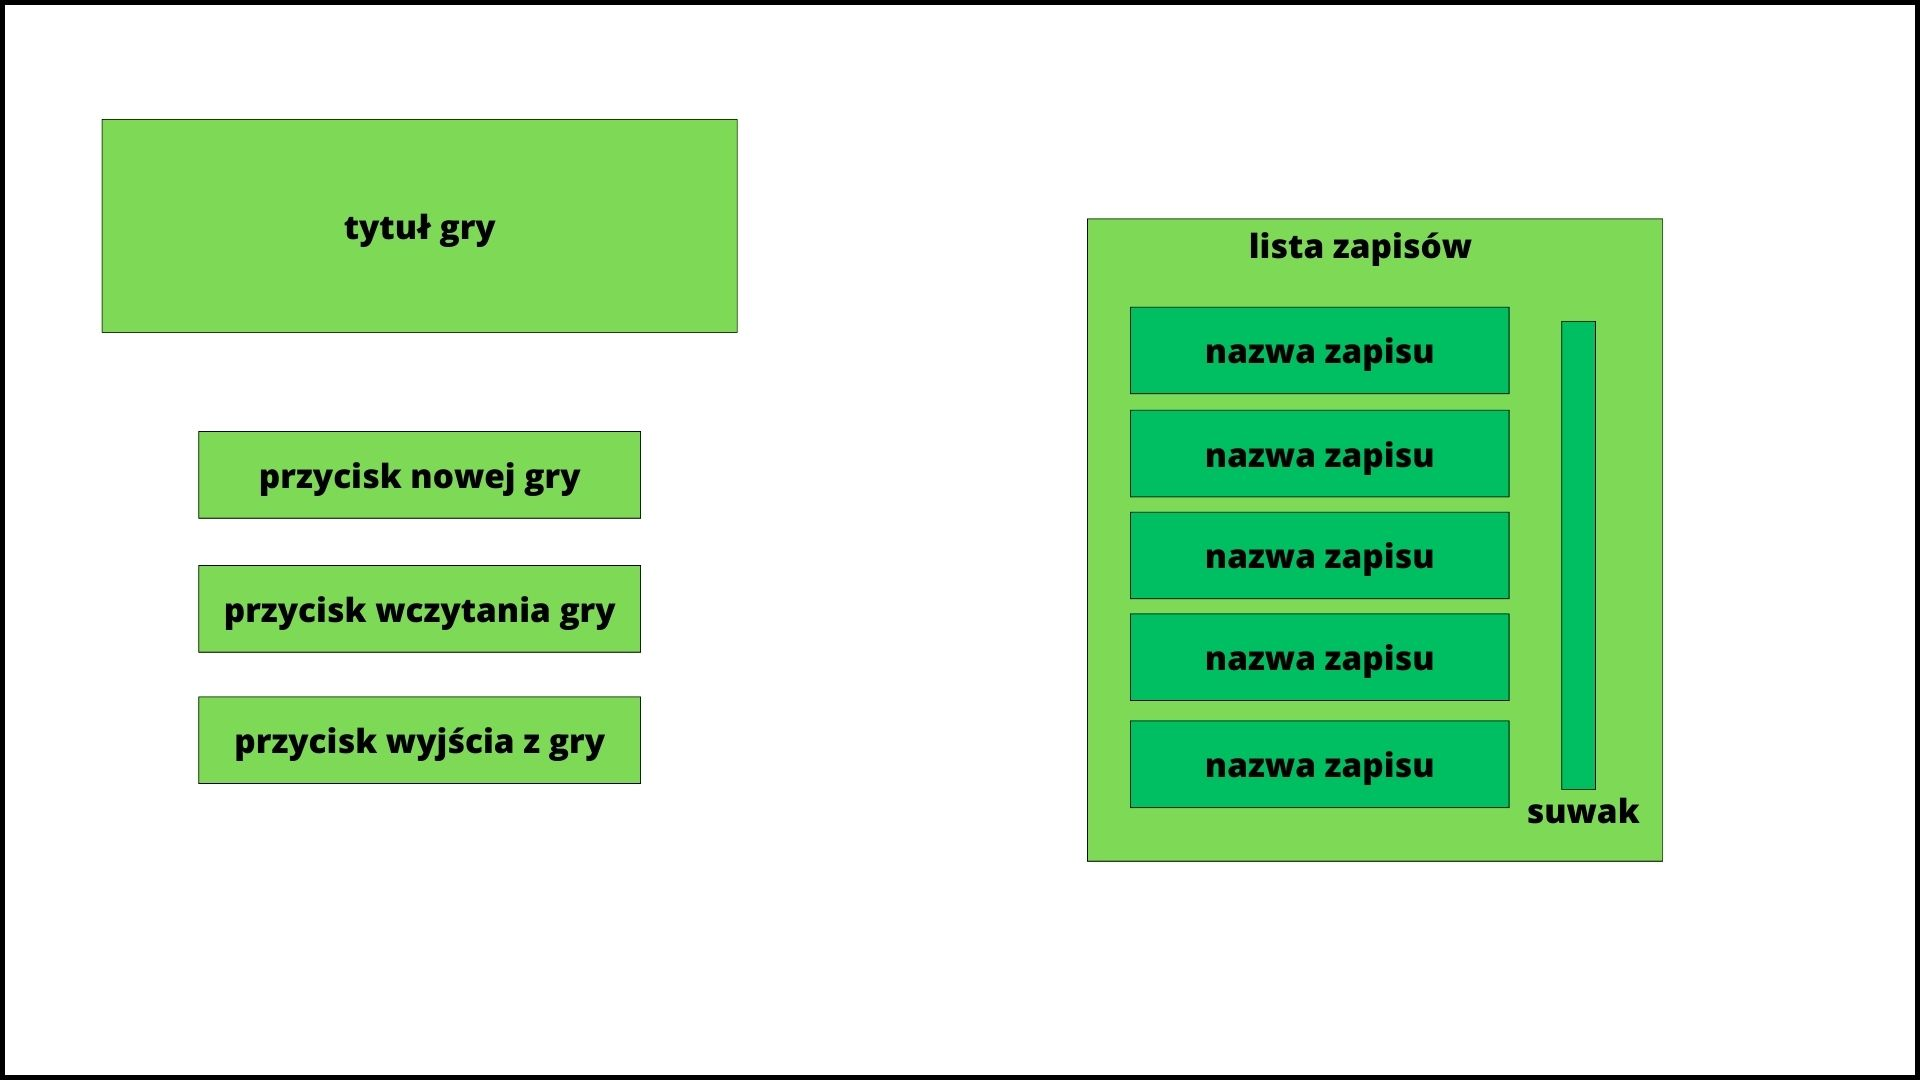
\includegraphics[width=0.8\textwidth]{images/ui/ui_prooj_menu.jpg}
    \caption{Projekt menu głównego.
    }\label{fig:compass}
\end{figure}

\section{Nawigacja (Zofia Sosińska)}\label{chap:naw}

Kluczowym dla gry założeniem jest ułatwienie graczowi wczucia się w realia świata, w którym się znajduje. 
Jako jeden z głównych warunków pogłębienia immersji uwypuklono brak implementacji mapy, na której gracz widziałby świat. 
W ten sposób nie upraszczamy mu poruszania się i odnajdywania lokacji tak,
jak i człowiek w realnym świecie w czasach średniowiecznych nie kierował się zapisanymi na kartce kartograficznymi obrazami, 
ale własną i zdobytą od innych wiedzą o otaczającym go terenie. 

Jedyną pomocą, jaką otrzyma gracz, będzie pasek obrazujący pole widzenia granej postaci.
Pierwszą rolą narzędzia będzie pokazanie kierunku świata, który znajduje się w polu widzenia gracza.
Zakładamy, że grana postać potrafi sama taką informację odczytać, chociażby z położenia Słońca.

Kolejną informacją na omawianym elemencie będzie miejsce, w którym znajduje się przeciwnik. 
Dotyczy to antagonistów widocznych w polu widzenia, jak i ukrytych za ścianą. 
Druga część będzie logicznie ponieważ zakładamy, że postać gracza może usłyszeć 
wroga za przeszkodą.


\section{Rozwój postaci gracza (Bartosz Strzelecki)}\label{s:proj_progres}
System rozwoju postaci jest inspirowany serią gier The Elder Scrolls (por. \ref{s:wpr_progres}) i będzie stanowił podstawowy element rozwoju toku rozgrywki.
Użytkownik będzie rozwijał umiejętności swojej postaci poprzez wykonywanie czynności związanych z daną statystyką.
Cechy, które gracz może rozwijać, korzyści, jakie z nich płyną, i sposób ich rozwoju przedstawia tabela \ref{fig:prog}.

\begin{table}[h]
\caption{Rozwijalne umiejętności gracza.}
\begin{center}
  \begin{tabular}{ | m{10em} | m{10em} | m{10em} | }
  \hline
    Statystyka & Sposób rozwoju & Korzyści \\
  \hline\hline
    Siła & Własnoręczne pokonywanie wrogich jednostek & Większa obrażenia zadawane przez postać gracza podczas uderzeń \\
    Przywództwo & Pokonywanie wrogich jednostek z użyciem pomocy przyjaznych wojowników & Większe obrażanie zadawane przez przyjazne jednostki \\
    Charyzma & Pomaganie mieszkańcom świata & Przychylniejsze efekty podczas rozmów z postaciami niezależnymi \\
  \hline
  \end{tabular}
\end{center}
\label{fig:prog}
\end{table}

\section{Mechanizm budowania (Bogna Lew)}\label{s:bud_impl}

Opracowany mechanizm umożliwia graczowi na przełączenie się w tryb budowania poprzez naciśnięcie klawisza \texttt{B}, który od razu
wyświetli podgląd bazowego obiektu. Widok budynku przemieszcza się przed postacią oraz odpowiednio obraca się razem z
nią. Efekt poruszania się podglądu został uzyskany za pomocą poniższego wzoru:
\begin{equation}
\begin{cases}
x = r \times sin(\alpha) \\
y = 0 \\
z = r \times cos(\alpha)
\end{cases}
\end{equation}

gdzie $x$, $y$ i $z$ to współrzędne odpowiednio względem osi X, Y i Z, $r$ to odległość środka obiektu od postaci
gracza, natomiast $\alpha$ to kąt o jaki jest on obrócony względem osi Y.

Podgląd budynku będzie widoczny do czasu, aż gracz go umieści naciskając prawy przycisk myszy bądź wychodząc z trybu
edycji naciskając klawisz \texttt{Escape}. Jeżeli widok budowli znajduje się w poprawnym do umieszczenia miejscu to jest on
podświetlany na zielono, w przeciwnym razie - na czerwono. Wybudowanie powoduje przywrócenie bazowych kolorów obiektu
oraz włącza wykrywanie kolizji z nim, dzięki czemu budynek poprawnie oddziałuje z otaczającym go środowiskiem.

\begin{figure}[h!]
    \centering
    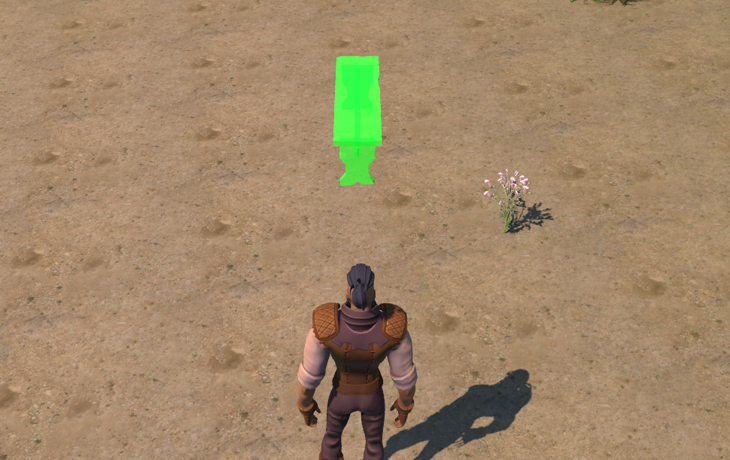
\includegraphics[width=1\textwidth]{images/implementacja/mechanizm_budowania/poprawne.png}
    \caption{Przykład podglądu w poprawnym umiejscowieniu.}
\end{figure}
\FloatBarrier

Do weryfikacji poprawności umiejscowienia budynku wykorzystano mechanizmy wyzwalacza (ang. \textit{trigger}) oraz rzucania
promienia (ang. \textit{raycasting}). Pierwszy z nich polega na wykrywaniu czy obiekt znalazł się w obszarze kolizji bez
brutalnego zatrzymywania go. Oznacza to, że może on przeniknąć przez inny element bez widocznych konsekwencji, jedynie
wysyłając sygnał, że dana sytuacja nastąpiła. Druga metoda natomiast polega na wypuszczeniu promienia o pewnej długości
w zadanym kierunku i sprawdzeniu, czy z czymś się zderzył.

Wyzwalacz został zastosowany do wykrywania kolizji z innymi obiektami na mapie, takimi jak postacie, czy elementy
scenerii niebędące terenem. W tym celu wykorzystano metody \verb|OnTriggerEnter()| i \verb|OnTriggerExit()|, które są wywoływane
odpowiednio gdy, dany obiekt znalazł się w obszarze kolizji innego elementu, bądź go opuścił. Każda z nich odpowiednio
zmienia poprzez zwiększenie bądź zmniejszenie wartości licznika kolizji obiektu. Jeżeli jego wartość jest różna od zera, tzn.
obiekt z czymś koliduje, to umiejscowienie jest uznawane za niepoprawne.

Drugi z mechanizmów został wykorzystany do sprawdzenia nachylenia podłoża. Efekt został osiągnięty poprzez rzucenie
promienia o niewielkiej długości z każdego z dolnych narożników obiektu i zliczeniu ile z nich wykryło kolizję z ziemią.
Brak wykrycia kolizji można zinterpretować jako zapadanie się bądź zbyt mocne lewitowanie danego narożnika nad
powierzchnią ziemi. Z tego powodu przyjęto, że jeśli co najmniej trzy z nich zderzyły się z podłożem, to umiejscowienie
jest poprawne.

\begin{figure}[h!]
    \centering
    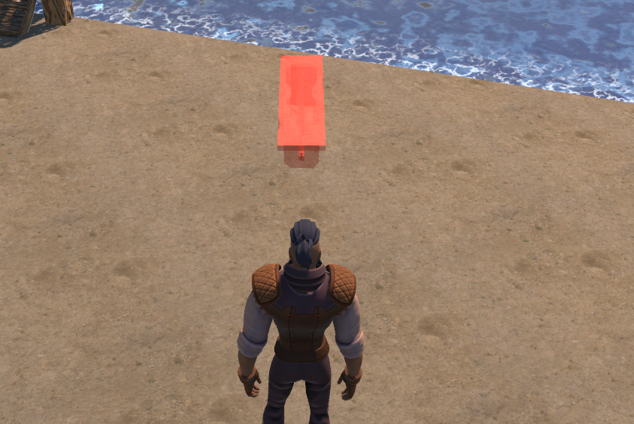
\includegraphics[width=1\textwidth]{images/implementacja/mechanizm_budowania/niepoprawne.png}
    \caption{Przykład podglądu w niepoprawnym umiejscowieniu.}
\end{figure}
\FloatBarrier

Dodatkowo metodę rzucania promienia wykorzystano do wykrycia kolizji z drzewami. Obiekty te są traktowane przez silnik
jako część terenu, przez co metoda wykorzystująca wyzwalacz pomija je. Dlatego w celu wykrywania kolizji z nimi
zdecydowano się na rzucenie dwóch grup promieni biegnących w głąb obiektu z naprzeciwległych krawędzi prostopadłych do
osi Y. Każdy z promieni biegnie w połowie wysokości obiektu i sięga przeciwnej ściany. Tak skomplikowany układ ma na
celu zapewnienie poprawności wykrywania kolizji w przypadku, gdy początki promieni znajdują się wewnątrz kolidującego
obiektu. Jeśli którykolwiek z nich zderzy się z drzewem, to wybrane miejsce jest uznawane za niepoprawne.

\begin{figure}[h!]
   \centering
   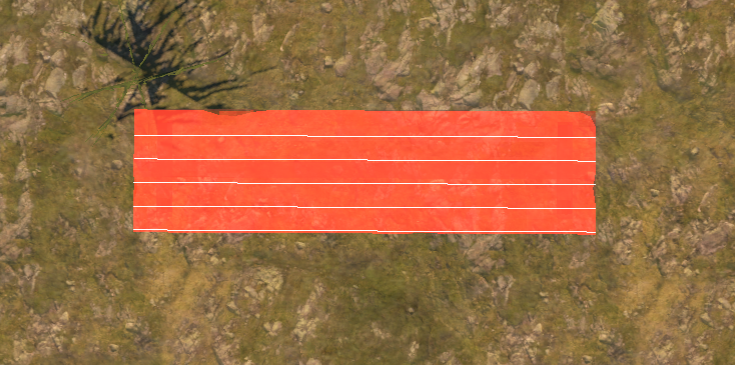
\includegraphics[width=1\textwidth]{images/implementacja/mechanizm_budowania/gizmos_drzewo_2.png}
   \caption{Widok z góry na siatkę promieni służących do wykrywania kolizji z drzewami.}
\end{figure}
\FloatBarrier
\begin{figure}[h!]
   \centering
   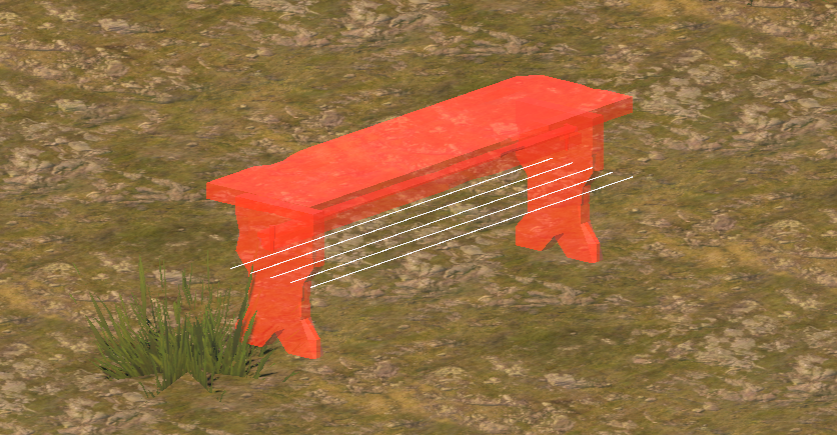
\includegraphics[width=1\textwidth]{images/implementacja/mechanizm_budowania/gizmos_drzewo_1.png}
   \caption{Widok z boku na siatkę promieni służących do wykrywania kolizji z drzewami.}
\end{figure}
\FloatBarrier

\section{Sterowanie jednostkami, podążanie za główną postacią (Zofia Sosińska)}\label{chap:sjpzgp}
Na samym początku gry stworzona przez gracza postać pojawia się sama. W tym momencie jest to jedyny obiekt, którym gracz może sterować.
Kontroluje, gdzie postać idzie, jak walczy oraz z kim rozmawia. Z biegiem czasu gra będzie jednak naciskać na formowanie drużyny,
ponieważ pokonywanie wielu przeciwników w pojedynkę będzie się stawało zbyt trudne. Pojawia się w takim momencie potrzeba 
zaimplementowania funkcjonalności zarządzania wieloma postaciami.

Stworzenie mechaniki poruszania się i oddziaływania na otaczający świat dla jednej postaci wydaje się proste i intuicyjne, ale kierowanie wieloma osobami już nie. 
Bez wprowadzenia zmian, używając jednego sposobu dyrygowania wszystkimi jednostkami tak samo, gra będzie prędko męczyć gracza.
Dla czynności małoznaczących, takich jak przemieszczenie drużyny w konkretne miejsce, wprowadzi monotonię i czasochłonność.
Każdą postać należy wybrać i przemieścić ją w konkretne miejsce. Kilka kliknięć przy jednej postaci jest akceptowalne, ale przy kilku wprowadzi to ogromne opóźnienia.

Jeszcze gorsze skutki pokazałyby się podczas walki. Szybkie przeskakiwanie pomiędzy postaciami podniosłoby zauważalnie trudność gry.
Poruszanie się jedną postacią i zabijanie przeciwników nie ma sensu, gdy reszta drużyny jest bita i nie może się obronić, ponieważ gracz musi się przełączyć na inną postać,
aby ta wykonała ruch. 

Z tego powodu potrzebny jest algorytm odpowiadający za właściwe poruszanie się pobocznych postaci.
Tworzona gra będzie dopuszczała małe, kilkunastoosobowe drużyny z przywódcą - postacią grywalną przez użytkownika - na czele.
Podczas walki graczowi pokażą się możliwe do wydania polecenia oraz specyfikacja, jakiej grupy mają one dotyczyć.
Za pomocą określonych klawiszy klawiatury będzie on mógł kontrolować zachowanie kompanów.

Po rozwiązaniu problemu mechaniki sterowania jednostkami w walce nie można przeoczyć samego poruszania się oraz interakcji ze światem.
Najprostszym rozwiązaniem będzie implementacja mechanizmu, według którego drużyna, po wykryciu znacznego przemieszczenia się przywódcy, sama będzie za nim podążać.
Kompani nie będą też mieli opcji samodzielnej interakcji ze światem, co sprawi, że poza walką zostaną jedynie biernymi obserwatorami.
\section{System dialogów. Bartosz Strzelecki}

System dialogów jest podstawową metodą, którą gracz będzie wykorzystywał, aby pozyskać informacje  o świecie oraz celach misji.
Gracz może inicjować konwersacje z postaciami niezależnymi, po czym zostaną mu zaproponowane opcje sposobu prowadzenia rozmowy.
W zależności od wybranych opcji dialogowych gracz może się spodziewać różnych konsekwencji.


\begin{figure}[h]
\centering

\includegraphics[width=0.6\textwidth]{images/fallout3}
\caption{Kadr z gry Fallout 3 przedstawiający przykładowy dialog}
\end{figure}

\href{https://assetstore.unity.com/packages/tools/utilities/dialogue-editor-168329}{Dialogue Editor} autorstwa Grasshop Dev jest prostym narzędziem pozwalającym na szybkie dodawanie i modyfikację dialogów.
Zawiera zestaw elementów ułatwiających wdrożenie systemu do projektu oraz udostępnia struktury danych wykorzystywanych do tworzenia interfejsu użytkownika.
Podczas rozmowy z postaciami niezależnymi gracz będzie mógł pozyskać informację o geografii świata, możliwych zagrożeniach oraz zadaniach do wykonania. 
Podobne systemy występują w grach takich jak Pillars of Eternity oraz w grach z serii Mass Effect.


\section{Sztuczna inteligencja (Bartosz Strzelecki)}\label{s:ai_impl}
Nawigacja przeciwników została zrealizowana poprzez wbudowany w silnik Unity system \texttt{NavMesh}. Pozwala on na łatwe wyznaczenie powierzchni, po której mogą poruszać
się postacie niekontrolowane przez gracza oraz realizuje zadanie wyznaczania ścieżki dla tych postaci.

\begin{figure}[h]
\centering
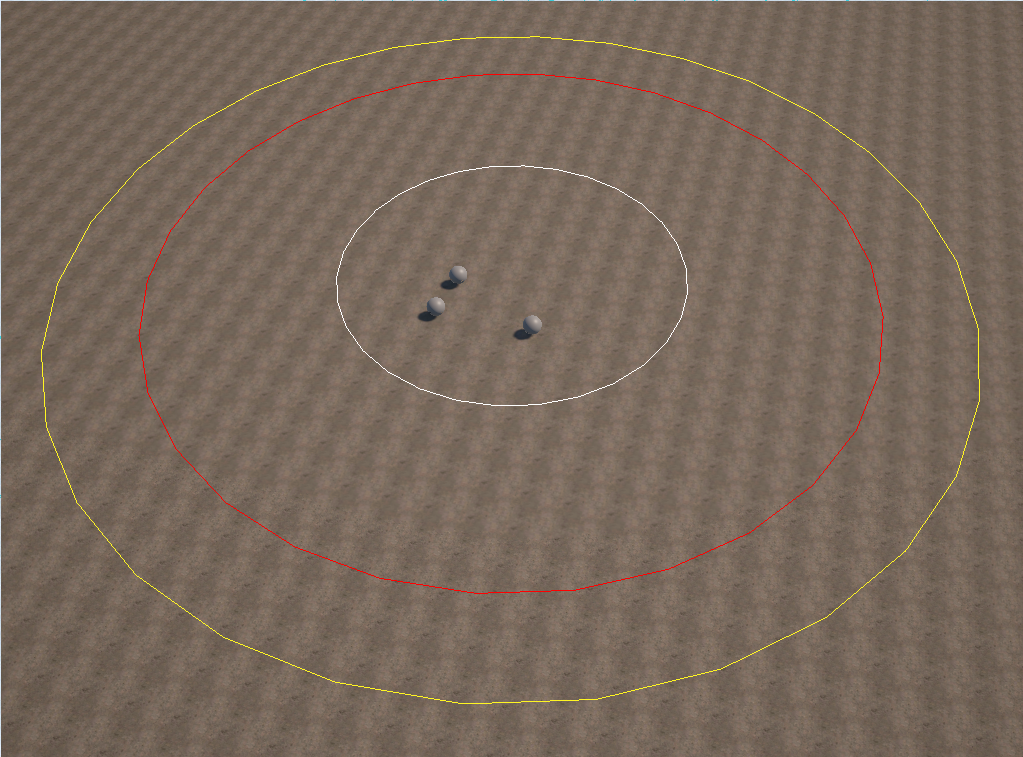
\includegraphics[width=0.9\textwidth]{images/ai}
\caption{Obraz przedstawia zasięgi odpowiednich regionów.}
\label{fig:regions}
\end{figure}
\FloatBarrier

Przeciwnicy są kontrolowani poprzez jeden obiekt przydzielający cele każdemu przypisanemu wrogowi. W normalnym trybie wrogowie poruszają się w sposób losowy
w obrębie wyznaczonej przestrzeni (biały okrąg na rys. \ref{fig:regions}). Kiedy przyjazne jednostki znajdą się w wystarczającej odległości (czerwony okrąg na rys. \ref{fig:regions}), przeciwnicy obiorą sobie za cel jedną z nich.
Po opuszczeniu przez drużynę gracza wyznaczonego obszaru (żółty okrąg na rys. \ref{fig:regions}) wrogowie wracają do poruszania się w sposób losowy w obrębie białego okręgu.


\begin{figure}[h]
\centering
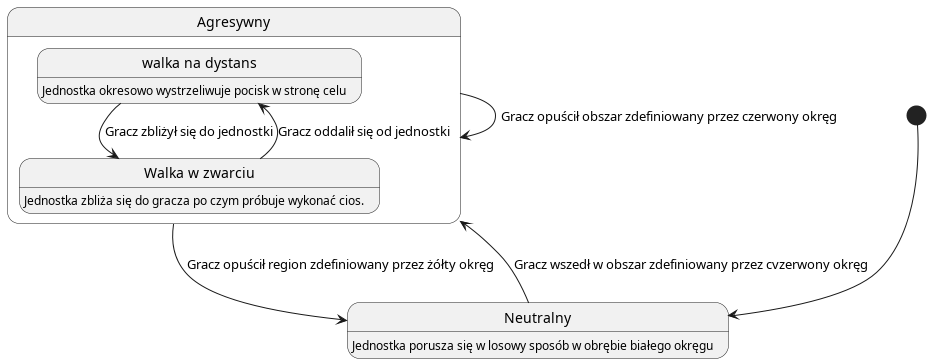
\includegraphics[width=1\textwidth]{uml/ai}
\caption{Diagram przedstawiający przepływ stanów dla sztucznej inteligencji przeciwników.}
\end{figure}
\FloatBarrier

\section{Widzenie przez horyzont (Bartosz Strzelecki)}\label{s:wid_impl}
Efekt został osiągnięty poprzez zmodyfikowanie potoku renderowania w taki sposób, że w zależności od wartości w buforze głębi jest wykorzystywany inny shader.
W tym przypadku, jeżeli sfera jest przysłonięta przez ścianę, jest ona narysowana, a w przeciwnym wypadku jest uruchamiany pusty shader.
"Unity domyślnie sortuje obiekty na podstawie odległości od kamery. Tak więc
w miarę zbliżania się obiektu do kamery, będzie on rysowany nad wszystkimi obiektami znajdującymi się dalej od kamery.
W większości przypadków sprawdza się to dobrze podczas tworzenia gier, ale
znajdą się sytuacje, w których będziemy chcieli mieć większą kontrolę nad sortowaniem obiektów na scenie. Używając bloku \verb|Tags\{\}| możemy kontrolować to sortowanie.
Unity udostępniło nam kilka domyślnych kolejek renderowania, z których każda ma unikalną wartość, którą
kieruje Unity, kiedy należy narysować obiekt na ekranie. Te wbudowane kolejki renderowania
nazywają się \verb|Background|, \verb|Geometry|, \verb|AlphaTest|, \verb|Transparent| i \verb|Overlay|." \cite{shaderscookbook}. Wykorzystując ten mechanizm
możliwe jest uzyskanie efektu widzenia przez postać gracza poprzez horyzont. Uzyskujemy przez to efekt podobny do tego zaimplementowanego w grze \textit{Dead by Daylight} (por. \ref{chap:dbd}).

Po naciśnięciu przycisku \texttt{E} następuje zagranie animacji opisanej wzorami

\begin{equation}
w(t, offset) = 1.1 \times 2.1^{-\left(\frac{{\left(\sin(t) + 1 - 0.4 - \text{{offset}}\right)^2}}{{0.02}}\right)}
\end{equation}

oraz

\begin{equation}
w(t, 0) - w(t, -0.2) + w(t, -1) - w(t, -1.2)
\end{equation}

Od podanych funkcji zależy przeźroczystość, jak i natężenie efektu Fresnela. 

\begin{figure}[h]
    \centering
    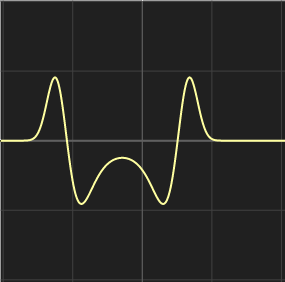
\includegraphics[width=0.5\textwidth]{images/g}
    \caption{Wykres przedstawiający funkcję opisującą natężenie efektu w animacji markera.}
\end{figure}



\begin{lstlisting}[language=C++, caption=Fragment shadera odpowiedzialny za animację.]
fixed4 frag (v2f i) : SV_Target
{
  float t =  6.2 * _Progress - 0.6;
  fixed4 pattern = tex2D(_PatternTex, i.uv + _Speed *t);
  float fresnelInfluence = dot(i.worldPos, i.viewDir);
  float saturatedFresnel = saturate(1 - fresnelInfluence);

  float g = w(t, 0) - w(t, -0.2) + w(t, -1) - w(t, -1.2);
  float4 color = pow(saturatedFresnel, g * _FresnelPow) * (_Color * _ColorIntensity) * pattern;
  color.a *= dot(i.worldPos, i.viewDir);
  return color;
}
\end{lstlisting}

\begin{figure}[h]
\centering
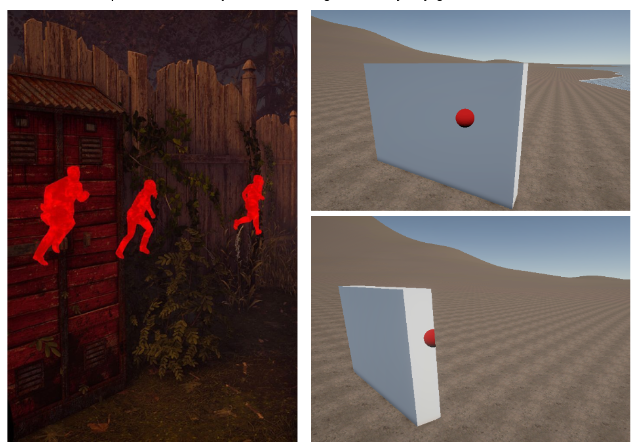
\includegraphics[width=0.6\textwidth]{images/shader}
\caption{Zachowanie programu cieniującego w przypadku przysłaniania markera przez przeszkody.}
\end{figure}

